\section{Interfaz gráfica}
\subsection{Conceptos básicos}
\begin{frame}{Conceptos básicos Android}
    \begin{block}{}Todos los componentes de la interfaz de usuario de Android descienden de la clase \textit{View}. Dichos objetos están organizados en forma de árbol y pueden contener nuevos objetos View, permitiendo crear interfaces muy completas.

Los objetos \textit{{View}}\index{View} se pueden definir de dos maneras:
\begin{itemize}
    \item {
    \pause
        Mediante un fichero XML colocado dentro del directorio \textit{{res/layout}}, que es el que usaremos normalmente.
    }
    \item <2->{
        En tiempo de ejecución, muy útil para crear nuestros propios componentes View.
    }
\end{itemize}
Para dibujar la interfaz, el sistema necesita que le pasemos el objeto View raiz, para ir descendiendo por cada uno de sus nodos y presentar al usuario toda la interfaz. El método encargado de esto es \textit{{Activity.setContentView()}}.\index{setContentView()}
    \end{block}
\end{frame}

\begin{frame}{Conceptos básicos Android}
    \begin{block}{}
Para que Android sepa dibujar correctamente los objetos, tenemos que pasarle algunos datos, como son la altura y anchura. Para eso nos servimos de la clase \textit{{LayoutParams}}\index{LayoutParams}, que puede tomar los siguientes valores:
    \begin{itemize}
    \item Un número. \pause
    \item <2-> La constante \textit{MATCH\_PARENT}\index{MATCH\_PARENT}, que indica que la vista debe intentar ser tan grande como su padre, quitando el padding.
    \item <3-> La constante \textit{WRAP\_CONTENT}\index{WRAP\_CONTENT}, para que intente ser lo suficientemente grande para mostrar su contenido, mas el padding.
    \end{itemize}
    \end{block}
\end{frame}

\begin{frame}{Conceptos básicos Android}
    \begin{block}{}
    Un atributo imprescindible es el \textit{{id}}(de tipo entero). Que sirve para identificar únicamente a un objeto View. Cuando lo declaramos mediante xml podemos referenciarlo a través de la clase de recursos R, usando una @.

    Los objetos View pueden tener otros muchos atributos, como padding, colores, imágenes, fondos, márgentes etc.
        \begin{itemize}
                \item \textit{\textbf{android:id=“@+id/nombreID”:}}
                Crea un nuevo atributo en la clase R llamado nombreID.\pause
                \item <2-> \textit{\textbf{android:id=“@id/nombreID”:}}
                Hace referencia a un id ya existente asociado a la etiqueta 'nombreID'.
                \item <3-> \textit{\textbf{android:id=“@android:id/list”:}}
                Referencia a un a etiqueta definida en la clase R del sistema llamada 'list'.
        \end{itemize}
    \end{block}
\end{frame}

\section{Layouts}

\begin{frame}{Qué es un layout}
    \begin{block}{}
Los layout\index{layout} nos permiten posicionar cada objeto gráfico en el lugar que queramos de la pantalla, es decir, nos permite diseñar el aspecto gráfico que va a tener nuestra pantalla. Los layouts son de tipo ViewGroup\index{ViewGroup}, una subclase de View\index{View}.

Existen varios tipos de Layouts para Android, vamos a ver los más comunes:
    \end{block}
\end{frame}

\subsection{LinearLayout}
\begin{frame}{LinearLayout}
    \begin{block}{}
    Este tipo de layout coloca sus hijos unos detrás de otros, comenzando por la esquina superior izquierda de la pantalla. Podemos colocarlos alineados horizontalmente o verticalmente mediante su propiedad \textit{{android:orientation=“horizontal | vertical”}}.
\begin{figure}[h]
    \centering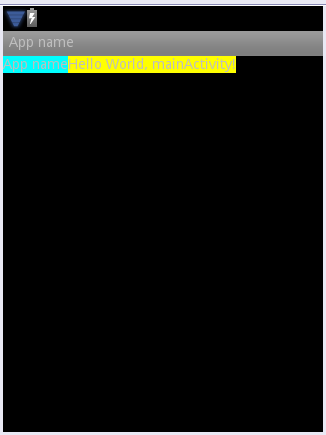
\includegraphics[scale=.35]{./img/LinearLayout.png}
    \caption{LinearLayout}
\end{figure}
\end{block}
\end{frame}

\begin{frame}[fragile]{LinearLayout}
    \begin{block}{}
\begin{xmlcode}
<linearlayout
    android:orientation="horizontal"
    android:layout_width="match_parent"
    android:layout_height="match_parent">

    <textview android:layout_width="wrap_content"
        android:layout_height="wrap_content"
        android:text="@string/app_name"
        android:background="#0ff"/>

    <textview android:layout_width="wrap_content"
        android:layout_height="wrap_content"
        android:text="@string/hello"
        android:background="#ff0"/>
</linearlayout>
\end{xmlcode}
    \end{block}
\end{frame}

\subsection{RelativeLayout}

\begin{frame}{RelativeLayout}
    \begin{block}{}
Este Layout permite que coloquemos los elementos en un lugar con respecto a la posición de otro, es decir, colocar un botón a la derecha de un texto, o centrarlo en la pantalla, o por ejemplo, colocar un texto encima de tal elemento y a la derecha de este otro.

Para conseguir esto, \textit{{RelativeLayout}} proporciona propiedades como \textit{{android:layout\_toRightOf}} o \textit{{android:layout\_alignLeft}}, que toman como valores los identificadores de los objetos, o valores booleanos.
    \end{block}
\end{frame}

\begin{frame}
    \begin{block}{}
\begin{figure}[H]
    \centering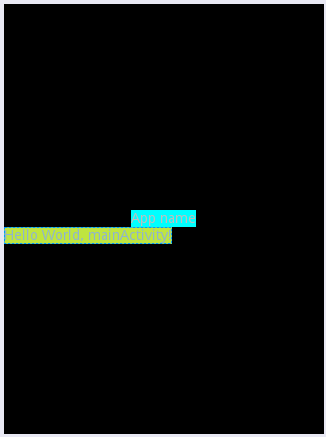
\includegraphics[scale=.45]{./img/RelativeLayout.png}
    \caption{RelativeLayout}
\end{figure}
    \end{block}
\end{frame}

\begin{frame}[fragile]{RelativeLayout}
    \begin{block}{}
\begin{xmlcode}
<relativelayout
    android:orientation="horizontal"
    android:layout_width="match_parent"
    android:layout_height="match_parent">
    <textview android:layout_width="wrap_content"
        android:layout_height="wrap_content"
        android:text="@string/app_name"
        android:background="#0ff"
        android:layout_centerInParent="true"
        android:id="@+id/text1"/>
    <textview android:id="@+id/text2"
        android:layout_width="wrap_content"
        android:layout_height="wrap_content"
        android:text="@string/hello"
        android:background="#ff0"
        android:layout_below="@id/text1"/>
</relativelayout>
\end{xmlcode}
    \end{block}
\end{frame}
